\chapter{Theoretical Background}

\section{ Convolution Neural Network - CNN }
Convolution Neural Networks are a special class of Neural Networks \cite{masood2018real}. They are made up
of neurons that have learnable weights and biases. Each neuron receives some inputs,
performs a dot product and optionally follows it with a non-linearity. CNN mainly consist
of Convolution Layers, Pooling Layers, Activation Layers and Fully Connected Layers.
ConvNet architectures make the explicit assumption that the inputs are images,
which allows us to encode certain properties into the architecture. These then
make the forward function more efficient to implement and vastly reduce the amount
of parameters in the network. Some of the main uses of CNN can be mentioned as: image
classification, object detection, semantic segmentation, face recognition, etc.

%Insert picture about CNN https://scholarworks.iupui.edu/bitstream/handle/1805/24768/FINAL%20Prasham_Shah_Thesis%20.pdf?sequence=1&isAllowed=y
\begin{figure}[H]
	\centering
	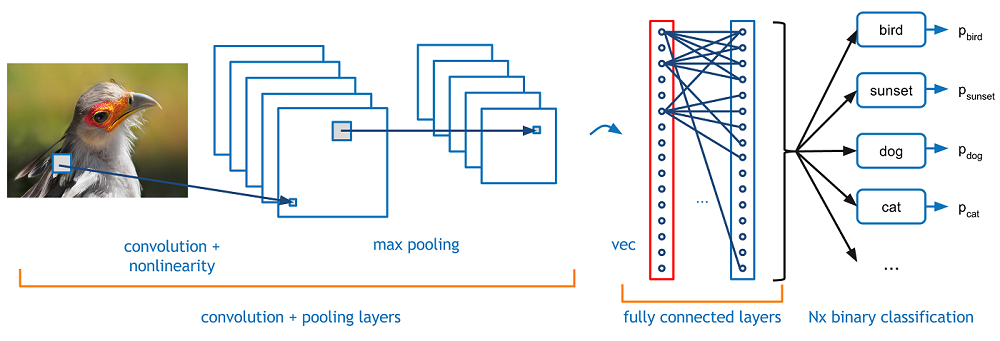
\includegraphics[width=\textwidth]{img/Chap3/Cover.png}
	\caption{Convolution Neural Network}
	\label{fig:Chap3-OverviewTheCNN}
\end{figure}
The figure \ref{fig:Chap3-OverviewTheCNN} above shows an example of convolution neural network, which is taking an image
as input and then extracting features from it through various layers and then finally predicting the
class of the object in the given image.

\subsection{ Architecture }
Convolution Neural Networks have a different architecture than regular Neural Networks, we can see
this different in figure \ref{fig:Chap3-DiffArchCNN_NNN} below.
Regular Neural Networks transform an input by putting it through a series of hidden layers.
Every layer is made up of a set of neurons, where each layer is fully connected to all neurons
in the layer before. Finally, there is a last fully-connected layer (the output layer) that
represent the predictions.
With CNN architecture. First of all, the layers are organized in
3 dimensions: width, height and depth. Further, the neurons in one layer do not connect to all
the neurons in the next layer but only to a small region of it. Lastly, the final output will
be reduced to a single vector of probability scores, organized along the depth dimension.
%FIXME: Insert image of diff architecture : https://www.freecodecamp.org/news/an-intuitive-guide-to-convolutional-neural-networks-260c2de0a050/
\begin{figure}[H]
	\centering
	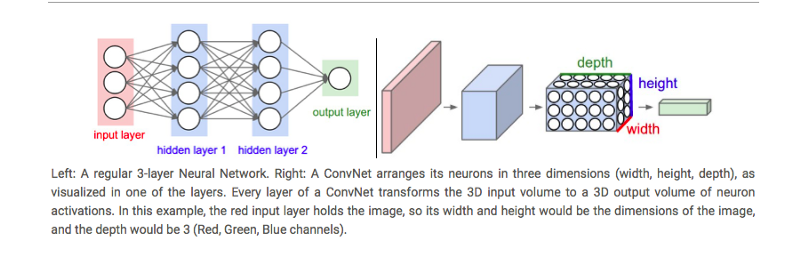
\includegraphics[width=\textwidth]{img/Chap3/DiffArchCNN-ANN}
	\caption{Different between Normal Neural Network and Convolution Neural Network}
	\label{fig:Chap3-DiffArchCNN_NNN}
\end{figure}
As we can see in figure \ref{fig:Chap3-CNN_Arch}. CNN can be divided into two parts:
%FIXME: Insert image of CNN arc: https://www.freecodecamp.org/news/an-intuitive-guide-to-convolutional-neural-networks-260c2de0a050/
\begin{figure}[H]
	\centering
	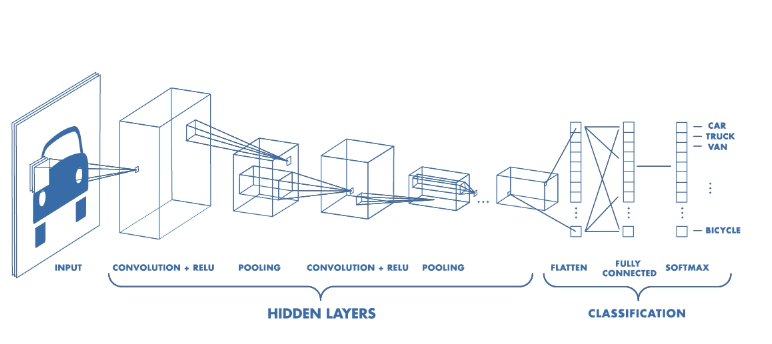
\includegraphics[width=\textwidth]{img/Chap3/CNN-Arch}
	\caption{Convolution Neural Network Architecture}
	\label{fig:Chap3-CNN_Arch}
\end{figure}

\begin{enumerate}
	\item The hidden layers/ Feature extraction part
	      \begin{itemize}
		      \item In this part, the network will perform a series of convolutions and
		            pooling operations during which the features are detected. If you had a
		            picture of a zebra, this is the part where the network would recognise
		            its stripes, two ears, and four legs.
	      \end{itemize}
	\item The Classification part
	      \begin{itemize}
		      \item Here, the fully connected layers will serve as a classifier on top of
		            these extracted features. They will assign a probability for the object
		            on the image being what the algorithm predicts it is.
	      \end{itemize}
\end{enumerate}

\subsection{ Feature extraction part }
\subsubsection{ Convolutional Layer }
Convolution Layer is the core building block of a Convolutional Network that does most
the computational heavy lifting. A convolution is executed by sliding the filter over
the input. At every location, a matrix multiplication is performed and sums the result onto
the feature map. This process of extracting features from image happens throughout the CNN's convolutional
layers. This process is illustrated in figure \ref{fig:Chap3-CNN_Layer}

% FIXME: https://scholarworks.iupui.edu/bitstream/handle/1805/24768/FINAL%20Prasham_Shah_Thesis%20.pdf?sequence=1&isAllowed=y
\begin{figure}[H]
	\centering
	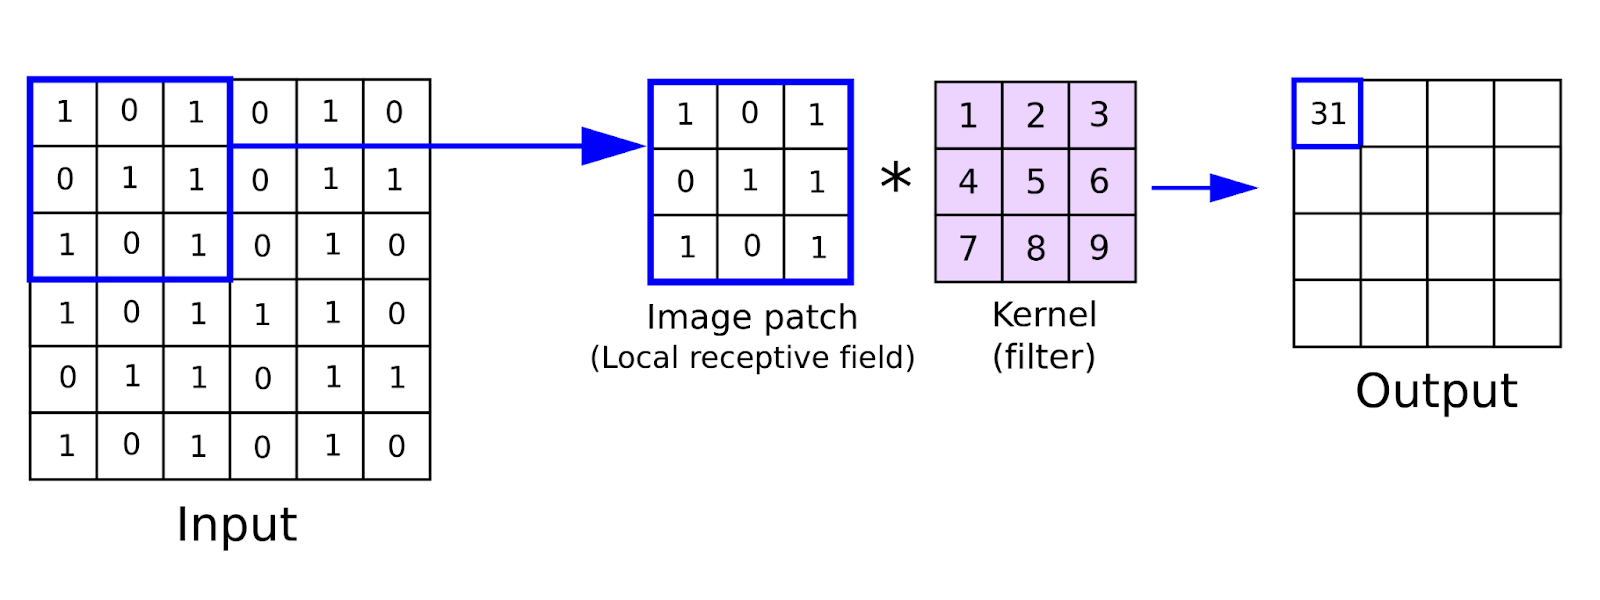
\includegraphics[width=\textwidth]{img/Chap3/ConvLayer}
	\caption{Convolution Neural Network Layer}
	\label{fig:Chap3-CNN_Layer}
\end{figure}
When the feature map is made, we can pass each value in
the feature map through a non-linearity function, such as ReLU, sigmoid, etc. Before it
becomes the input of the next convolution layer.

Because the size of the feature map is always smaller than the input, we have
to do something to prevent our feature map from shrinking. This is where we use
padding (\ref{fig:Chap3-CNN_Padding}). A layer of zero-value pixels is added to surround the input with zeros,
so that our feature map will not shrink. In addition to keeping the spatial
size constant after performing convolution, padding also improves performance
and makes sure the kernel and stride size will fit in the input.
% FIXME: => Need picture
\begin{figure}[H]
	\centering
	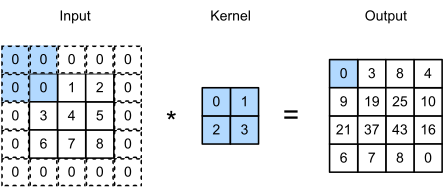
\includegraphics[width=\textwidth]{img/Chap3/CNN_Padding}
	\caption{Using padding for strike one in Convolution Layer}
	\label{fig:Chap3-CNN_Padding}
\end{figure}
\subsubsection{ Pooling Layers }
After a convolution layer, it is common to add a pooling layer in between CNN layers.
The function of pooling is to continuously reduce the dimensionality to reduce the number
of parameters and computation in the network. This shortens the training time and controls
overfitting.

There are mainly two types of Pooling Layers in a CNN: Max Pooling and Average
Pooling. The functionality of these two types of layers are demonstrated in figure \ref{fig:Chap3-CNN_Pooling} .
Max Pooling restores the maximum value from the segment of the picture covered
by the Kernel. Whereas, Average Pooling restores the average of the multitude of
values from the bit of the picture covered by the Kernel.

\begin{figure}[H]
	\centering
	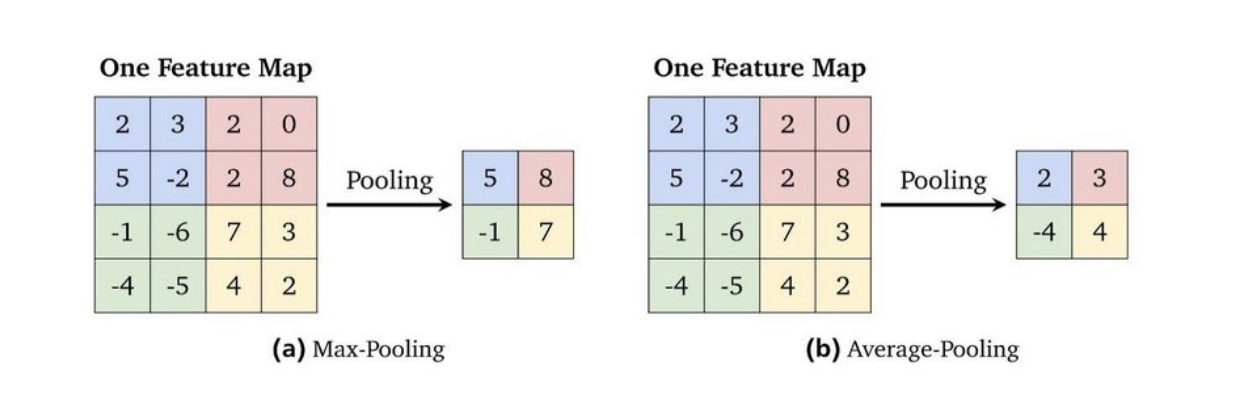
\includegraphics[width=\textwidth]{img/Chap3/Pooling}
	\caption{Max Pooling and Average Pooling}
	\label{fig:Chap3-CNN_Pooling}
\end{figure}

% FIXME: Insert image about max pooling and average pooling

\subsubsection{ Activation Layers }
Neural networks in general and CNNs in particular rely on a non-linear "trigger" function
to signal distinct identification of likely features on each hidden layer. CNNs may use a
variety of specific functions (figure \ref{fig:Chap3-CNN_ActiveFunction}), such as rectified linear
units (ReLUs) and continuous trigger (non-linear) functions—to efficiently implement this non-linear triggering.
\begin{figure}[H]
	\centering
	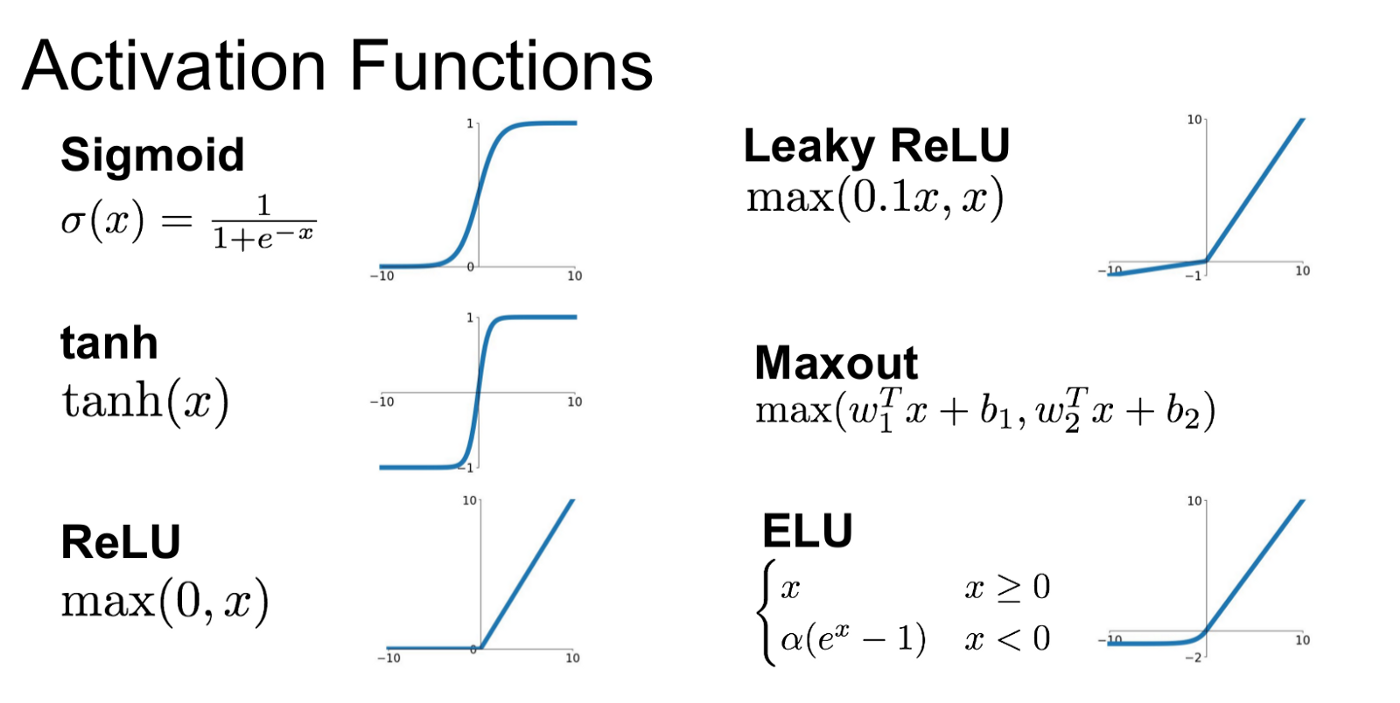
\includegraphics[width=\textwidth]{img/Chap3/ActiveFunction}
	\caption{ Some Active Function common used in CNN }
	\label{fig:Chap3-CNN_ActiveFunction}
\end{figure}
% FIXME: Insert picture of some function like ReLU, tanh ....
\subsection{ Classification part }
\subsubsection{ Fully connected layers }
The last layers of a CNN are fully connected layers. Neurons in a
fully connected layer have full connections to all the activations in the previous
layer. This part is in principle the same as a regular Neural Network.

Figure \ref{fig:Chap3-FC} illustrates the way of input value stream into the fully connected layer.
Because these fully connected layer can only accept one dimensional data. So, we need convert our 3D
data to 1D data. After pass through some FC, we will get the result is the data
classification.

\begin{figure}[H]
	\centering
	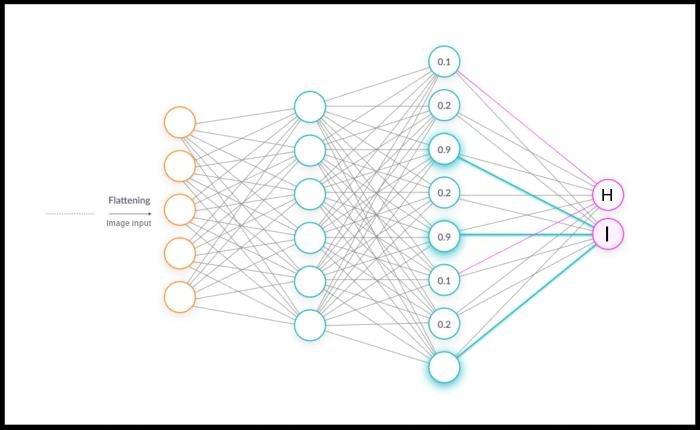
\includegraphics[width=\textwidth]{img/Chap3/FC}
	\caption{ Fully connected Layer}
	\label{fig:Chap3-FC}
\end{figure}
% FIXME: Insert picture ...
\section{ Media Pipe}\label{sec:MediaPipe}
% FIXME: Lấy từ eureka bỏ vào
\subsection{Introduction to Media Pipe Hands}
MediaPipe Hands (\ref{fig:Chap3-MediaPipe}) is a high-resolution tracking system for hands and fingers \cite{zhang2020mediapipe}. It uses machine learning to infer 21 3D hand landmarks from a single frame. This solution delivers real-time performance on a cell phone and even scales to many hands, whereas current state-of-the-art systems rely primarily on powerful desktop environments for inference.

\begin{figure}[H]
	\centering
	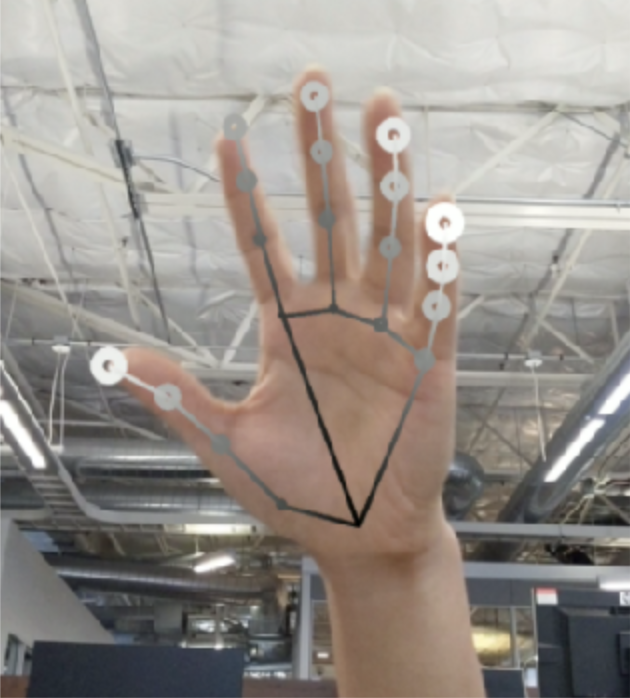
\includegraphics[width=0.8\textwidth]{img/Chap3/Media Pipe}
	\caption{ Media Pipe real time tracking 3D hand landmarks}
	\label{fig:Chap3-MediaPipe}
\end{figure}

MediaPipe Hands makes use of a machine learning pipeline that consists of several models that work together: A palm detection model, which acts on the entire image, will return an orientated hand bounding box. A hand landmark model that returns high-fidelity 3D hand key points from the cropped image region determined by the palm detector.

However, providing the hand landmark model with a correctly cropped hand image minimizes the requirement for data augmentation drastically (such as rotations, translations, and scaling) and instead allows the network to focus on coordinate prediction accuracy. Furthermore, in this ML pipeline, crops can be created based on the hand landmarks recognized in the previous frame, and palm detection is only used to localize the hand when the landmark model can no longer detect its presence.
\subsection{ Palm detection model }
The Media Pipe team provides the palm detection model to detect initial hand locations and distinguish whether the hand recognized is left or right, which is very useful as each sign goes along with a different side will result in different meanings. They created a single-shot detector model, comparable to the face detection model in MediaPipe Face Mesh \cite{MediaPipeFaceMesh}, tailored for mobile real-time applications. Hand detection is difficult: our model must detect occluded and self-occluded hands and work across many hand sizes with a significant scale span relative to the image frame.

According to their statement, the methods they use to address the above challenges vary in many strategies. First, instead of training a hand detector, they train a palm detector because estimating bounding boxes of inflexible objects like palms and fists is much easier than recognizing hands with articulated fingers. Furthermore, the non-maximum suppression method performs effectively even in two-hand self-occlusion situations such as handshakes because palms are small objects. Furthermore, palms can be simulated using square bounding boxes (anchors in ML language) that ignore other aspect ratios, reducing 3-5 anchors. Second, even for tiny objects, an encoder-decoder feature extractor is used for more extensive picture context awareness (similar to the Retina Net approach). Finally, the significant scale variance limits focus loss during training to support many anchors.

Using the strategies described above gives an average precision of 95.7 percent in palm detection. With no decoder and a regular cross-entropy loss, the baseline is just 86.22 percent.

\subsection{ Hand landmark model }
Following palm detection over the entire image, our next hand landmark model uses regression to accomplish exact key point localization of 21 3D hand-knuckle coordinates (see figure \ref{fig:Chap3-HandLandMark}) within the detected hand regions, i.e., direct, coordinate prediction. Even with partially visible hands and self-occlusions, the model develops a consistent internal hand posture representation.
\begin{figure}[H]
	\centering
	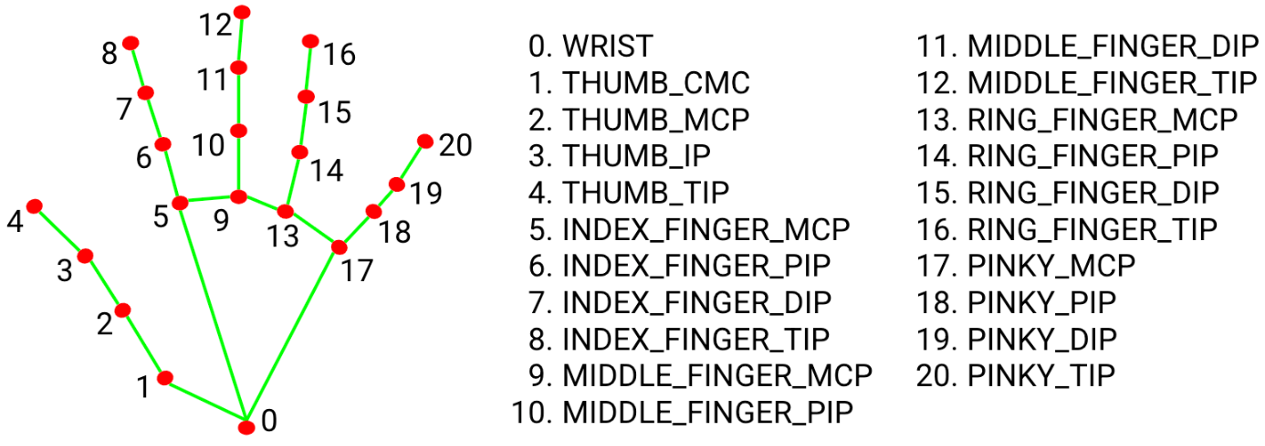
\includegraphics[width=\textwidth]{img/Chap3/HandLandMark}
	\caption{ 21 Hand Landmarks }
	\label{fig:Chap3-HandLandMark}
\end{figure}


\section{ Distance Matrix }
A distance matrix \cite{DistanceMatrix} is a table that shows the distance between pairs of objects.
For example, in the figure \ref{fig:Chap3-DM}., we can see the distance of A and B is 16, B and C is 37
and so on. In the diagonal of table is the distance of object from itself, so the value
as we can see is 0. Distance matrices are sometimes called dissimilarity matrices.

\begin{figure}[H]
	\centering
	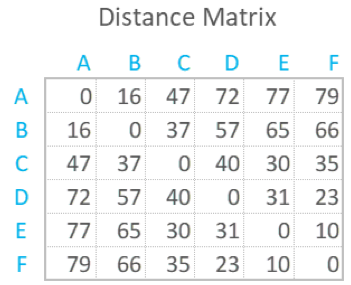
\includegraphics[width=0.6\textwidth]{img/Chap3/DM}
	\caption{ Distance Matrix }
	\label{fig:Chap3-DM}
\end{figure}

% FIXME: Insert picture of distance matrix

\subsection{ Create Distance Matrix }
A distance matrix is computed from a raw data table. In the example below (\ref{fig:Chap3-DM_Formula} ), we can use high school math (Pythagoras) to work out
that distance between A and B.

% FIXME: Chèn công thức vào đây
\begin{figure}[H]
	\centering
	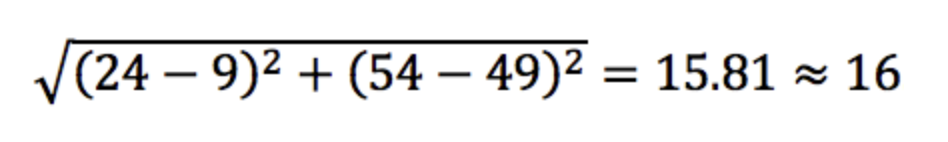
\includegraphics[width=0.7\textwidth]{img/Chap3/DM_Formula}
	\caption{ Calculating distance between A and B}
	\label{fig:Chap3-DM_Formula}
\end{figure}

We can use same formula with more than two variables, and this is known as
the Euclidean distance.
In result, we have the distance matrix represented like figure \ref{fig:Chap3-DM-Raw}
% FIXME: chèn bảng kết quả vào
\begin{figure}[H]
	\centering
	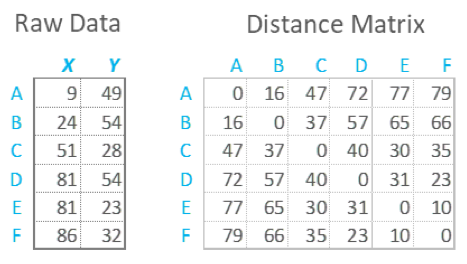
\includegraphics[width=0.7\textwidth]{img/Chap3/DM-Raw}
	\caption{ The Distance Matrix is constructed from Raw Data }
	\label{fig:Chap3-DM-Raw}
\end{figure}

\section{ Beam search and Connectionist Temporal Classification }
% CheckList:
%   [x] BeamSearch
%   [x] CTC recap
%   [x] Combination
%   [x] Pseudo code
\subsection{ Connectionist Temporal Classification }
Connectionist Temporal Classification (CTC) \cite{hannun2017sequence} is a type of Neural Network output helpful
in tackling sequence problems like handwriting (figure \ref{fig:Chap3-Overview-CTC}) and speech recognition where the timing varies.
Using CTC ensures that one does not need an aligned dataset, which makes the training process
more straightforward.
% FIXME: Insert about CTC in speech recognition
\begin{figure}[H]
	\centering
	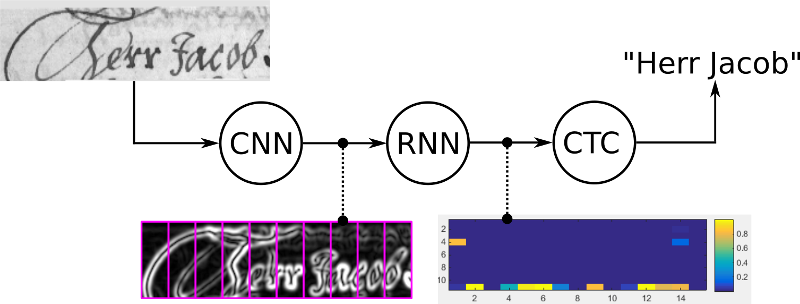
\includegraphics[width=\textwidth]{img/Chap3/Overview-CTC}
	\caption{ Overview of a Neural Network for handwriting recognition }
	\label{fig:Chap3-Overview-CTC}
\end{figure}

\subsection{ Why we want to use CTC }
In context of hand written recognition, we could create a data-set with
images of text-lines, and then specify for each horizontal position of the image
the corresponding character as shown in figure \ref{fig:Chap3-Annottion-image-CTC} Then, we could train a model to output
a character-score for each horizontal position. However, there are two problem with this
solution.
\begin{itemize}
	\item It takes a lot of time, annotating dataset at the character level is a boring task.
	\item What if the character takes up more than one time-step ?. We could get "tooo" because
	      the "o" is a wide character as shown in figure \ref{fig:Chap3-Annottion-image-CTC}. We have to remove all duplicate character
	      like "t" and "o".
\end{itemize}

% FIXME: Insert image ...
\begin{figure}[H]
	\centering
	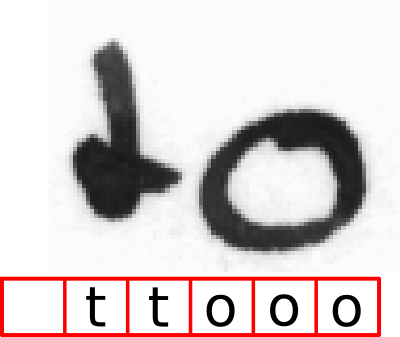
\includegraphics[width=0.6\textwidth]{img/Chap3/Annotation-image-CTC}
	\caption{ Annotation for each horizontal position of the image }
	\label{fig:Chap3-Annottion-image-CTC}
\end{figure}
CTC can solves both problem for us:
\begin{itemize}
	\item We can ignore both the position and width of the character in the image
	      and only requires the text that occurs in the image.
	\item Using decode techniques, we can directly get the result of the network and
	      no further post-processing of the recongnized text is needed.
\end{itemize}

\subsection{ Beam Search with CTC decoder }
CTC has more than Decoding phase, it can have the Encoding, Loss calculation, but in
this graduation thesis scope, we don't need it anymore. So, in here, we only
mention to CTC decoder but in the way of it combines with Beam Search \cite{scheidl2018word}. Because CTC
in decoding context, it can combine with another algorithm like best-path decoding, etc...

\subsubsection{ Beam search }
In computer science, beam search \cite{BeamSearch} is a heuristic search algorithm that
explores a graph by expanding the most promising node in a limited set.
Beam search is an optimization of best-first search the reduces its memory
requirements. Best-first search is a graph search which orders all
partial solutions (states) according to some heuristic. But in beam search,
only a predetermined number of best partial solutions are kept as candidates.
Pseudo-code for basic version of beam-search is shown is figure \ref{fig:Chap3-Basic-Version-BeamSearch}

\begin{figure}[H]
	\centering
	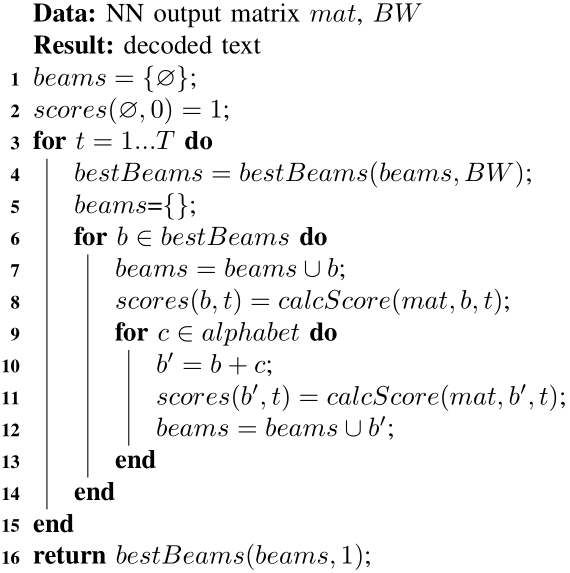
\includegraphics[width=0.8\textwidth]{img/Chap3/Basic-Version-BeamSearch}
	\caption{ Basic version of Beam Search }
	\label{fig:Chap3-Basic-Version-BeamSearch}
\end{figure}

% FIXME: Insert image about pseudo-code for beam-search

Beam search algorithm will be implemented through the following steps, with two
parameter will be included: output matrix and beam width (BW) which specifies the number
of beams to keep . First of all, the list of beam and corresponding score is
initialized (line 1 and 2). After that, from 3-15, the algorithm will loop over all time-steps
of the matrix output. At this point, only the best scoring beams (equal BW) from the previous
time-step are kept (line 4). Each of beam, we calculate the score and get result (line 8), we will cover
this step in more detail later. Further, each beam is extended by all possible characters from
the alphabet (line 10) and again, a score is calculated (line 11). After the last time-step,
the best beams is returned as a result (line 16).

% FIXME: Insert image about beam search

\begin{figure}[H]
	\centering
	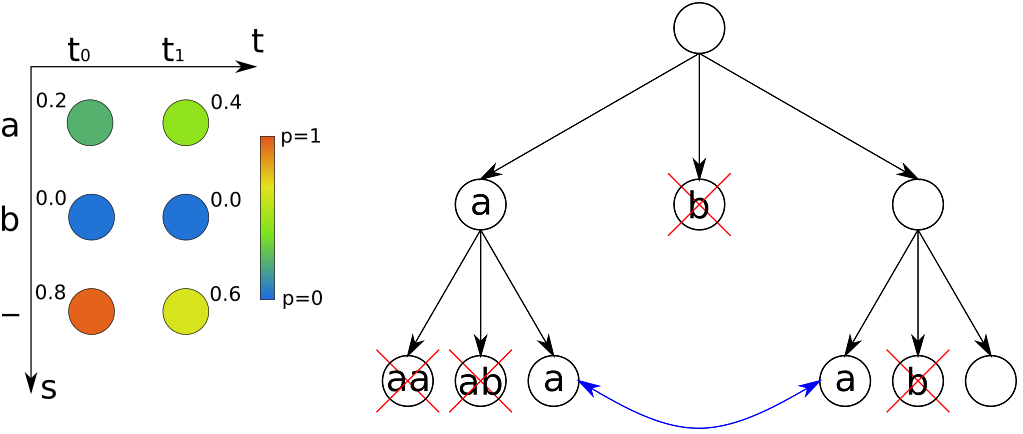
\includegraphics[width=\textwidth]{img/Chap3/BeamSearchTree}
	\caption{ NN output and tree of beams with alphabet = {"a", "b"} and BW = 2 }
	\label{fig:Chap3-BSTree}
\end{figure}

As we can see, in figure \ref{fig:Chap3-BSTree}, both output matrix to be decoded and the tree of beams are shown.
Beam search algorithm extended as possible and keep exactly BW candidates . Finally,
we finished the last iteration and the final step of the algorithm is to return the beam
with the highest score, which is "a" in this example.

\subsubsection{ Calculating the score }
As we just discuss above, in this part, we will talk about how to scoring the beam.
We will split the beam-score into the score of paths ending with a blank(e.g.. 'aa-')
and paths ending with non-blank (e.g. 'aaa').
\begin{itemize}
	\item We denote the probability of all paths ending with a blank and corresponding to a beam b at time-step t
	      by Pb(b,t) and by Pnb(b,t) for the non-blank case.
	\item The probability Ptot(b,t) of a beam b at time-step t is simply the sum of Pb and Pnb, for example:
	      Ptot(b,t) = Pb(b,t) + Pnb(b,t)
\end{itemize}

\begin{figure}[H]
	\centering
	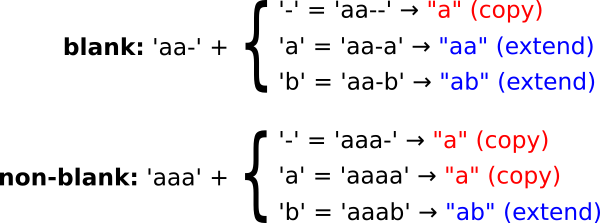
\includegraphics[width=0.7\textwidth]{img/Chap3/CTC_Scoring}
	\caption{ The effect of appending a character to paths ending with blank and non-blank }
	\label{fig:Chap3-CTC_Scoring}
\end{figure}

In figure \ref{fig:Chap3-CTC_Scoring}, we will see what happens when we extend a path. Three main case we can mention
is:
\begin{itemize}
	\item Extend by blank ('a' + '-' = 'a-')
	\item Extend by repeating last character ( 'aa' + 'a' = 'aaa' or 'aa-' + 'a' = 'aa-a')
	\item Extend by some other character ('aa' + 'b' = 'aab')
\end{itemize}

% FIXME: Viết lại các công thức bên dưới
And when we collapse the extended paths, two result we will get and some case we needed to handle:
\begin{itemize}
	\item The unchanged (copied) beam ('a' $ \rightarrow $ 'a'):
	      \begin{itemize}
		      \item To copy a beam, we can extend corresponding paths by a blank and get
		            paths ending with a blank: $ P_b (n, t) += P_{tot}(b, t-1)*mat(blank, t) $
		      \item Beside, with non-blank ending paths case, if we extend it by the last
		            character (the beam is not empty): $ P_{nb}(b,t) += P_{nb}(b,t-1)*mat(b[-1],t) $
		            with -1 indexes the last character in the beam
	      \end{itemize}
	\item An extended beam ('a' $\rightarrow$ 'aa' or 'ab'):
	      \begin{itemize}
		      \item To extend a beam. With the last character is different from the character we need
		            to extend, then there is no need for separating blanks ('-') in the paths:
		            $ P_{nb}(b+c,t) += P_{tot}(b,t-1)*mat(c,t) $
		      \item Or the last character of beam is repeated, we must ensure that the paths
		            end with a blank: $ P_{nb}(b+c,t) += P_b(b,t-1)*mat(c,t) $
		      \item We don't need t care about Pb(b+c,t) because we added a non-blank character
	      \end{itemize}
\end{itemize}

\subsubsection{ Putting it all together }
Figure \ref{fig:Chap3-BS_CTC} depicts the CTC beam search algorithm. It is similar to the basic version
previously displayed. However, it includes the code to score the beams: copied beams
(lines 7-10) and extended beams(line 15-19). Finally, when we looking for the best scoring
beams, the programs ranks them according to Ptot (line 4) and then take the BW best ones.

\begin{figure}[H]
	\centering
	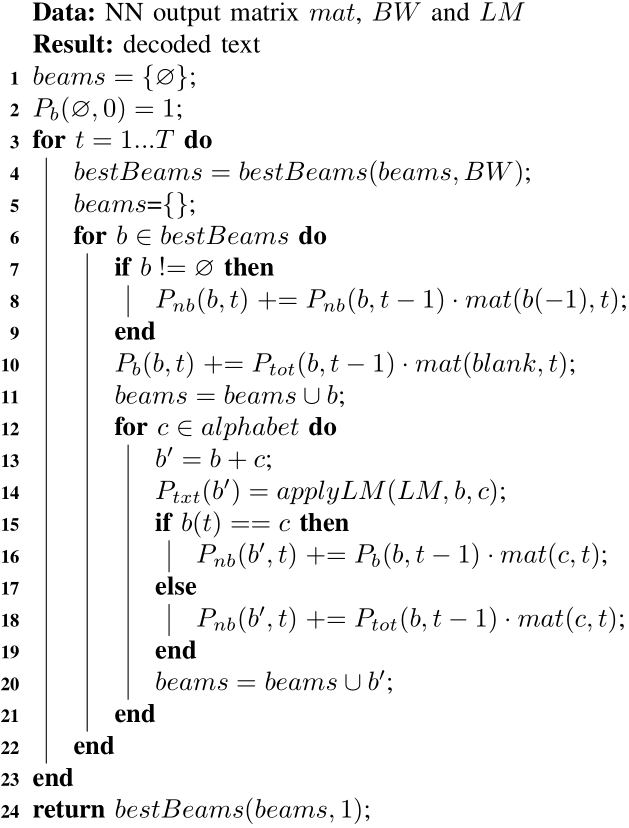
\includegraphics[width=0.8\textwidth]{img/Chap3/BS_CTC}
	\caption{ CTC beam search }
	\label{fig:Chap3-BS_CTC}
\end{figure}

